\documentclass[a4paper,12pt]{article}
\usepackage{indentfirst}
\usepackage{amsmath}
\usepackage{algorithm}
\usepackage[margin=1.1in]{geometry}
\usepackage[noend]{algpseudocode}
\usepackage{amssymb}
\usepackage{enumerate}
\usepackage{mathtools}
\usepackage{calligra}
\usepackage{tikz}
\usepackage{tikz,fullpage}
\usetikzlibrary{arrows,%
	petri,%
	topaths}%
\usepackage{tkz-berge}
\usepackage[position=top]{subfig}
\usetikzlibrary {positioning}
\usetikzlibrary{calc}

\title{ALGORITMICA GRAFURILOR \\
		Tema 2}
\author{Daniș Ciprian\\
		Oloieri Alexandru \\
		Anul II, Grupa A2}
\date{22 noiembrie 2019}

\begin{document}
	
\maketitle

\section{Problema 1}

\subsection{a)}

Fie $M \subset E(G), M \neq \varnothing$ mulțimea muchiilor de cost minim. 

\textbf{I}: Dacă interpretăm afirmația \textbf{a)} ca "Toți $m \in M$ sunt conținuți într-un arbore parțial de cost minim.", atunci, conform exemplului de mai jos:

\begin{center}
	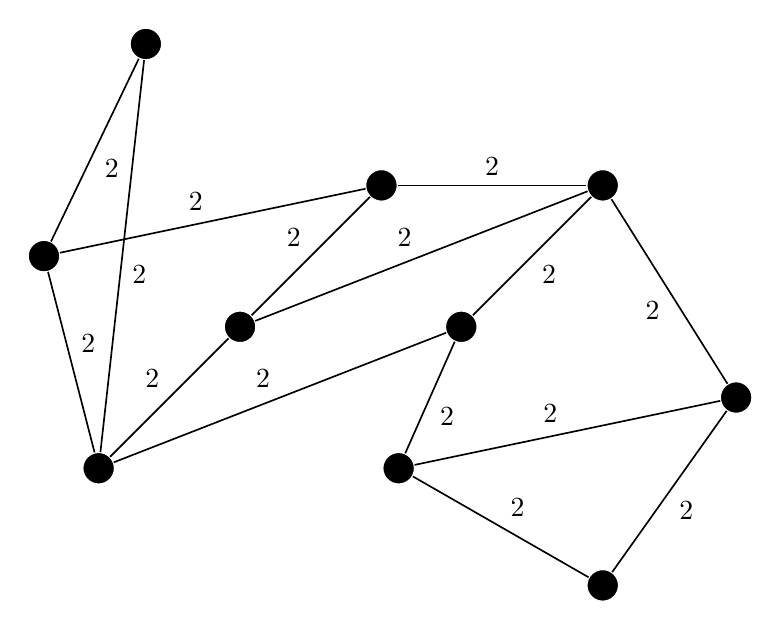
\begin{tikzpicture}[auto, node distance = 1.5in, on grid, state/.style = {circle, top color = black, bottom color = black, draw, white, text = black, minimum width = 4mm}]
	\node[state] (A) {};
	\node[state] (B) [below left = of A, xshift = 1.4cm] {};
	\node[state] (C) [below right = of B, xshift = -2cm] {};
	\node[state] (D) [node distance = 1in, above right = of C] {};
	\node[state] (E) [node distance = 1in, above right = of D] {};
	\node[state] (F) [right = of E, xshift = -1cm] {};
	\node[state] (G) [node distance = 1in, below left = of F] {};
	\node[state] (H) [node distance = 1in, below left = of G, xshift = 1cm] {};
	\node[state] (I) [below right = of F, xshift = -1cm] {};
	\node[state] (J) [node distance = 2in, below = of F] {};
	\draw[semithick] (A) -- node[auto]{2} (B);
	\draw[semithick] (B) -- node[auto]{2} (C);
	\draw[semithick] (A) -- node[auto]{2} (C);
	\draw[semithick] (B) -- node[auto]{2} (E);
	\draw[semithick] (C) -- node[auto]{2} (D);
	\draw[semithick] (D) -- node[auto]{2} (E);
	\draw[semithick] (D) -- node[auto]{2} (F);
	\draw[semithick] (E) -- node[auto]{2} (F);
	\draw[semithick] (C) -- node[auto]{2} (G);
	\draw[semithick] (F) -- node[auto]{2} (G);
	\draw[semithick] (G) -- node[auto]{2} (H);
	\draw[semithick] (H) -- node[auto]{2} (I);
	\draw[semithick] (H) -- node[auto]{2} (J);
	\draw[semithick] (I) -- node[auto]{2} (J);
	\draw[semithick] (I) -- node[auto]{2} (F);
	\end{tikzpicture}
\end{center}

Avem că $M = E(G), c(m) = 2,\forall m \in M$, dar cum un arbore parțial conține doar $n-1$ muchii $(n=10 \text{ în exemplu})$, vom avea că nu toate muchiile din $M$ intră într-un $T \in \text{{\calligra T}}_G$ de cost minim $\Rightarrow$ afirmația \textbf{a)} este falsă.

\textbf{II}: Dacă interpretăm afirmația \textbf{a)} ca "Toți $m \in M$ sunt conținuți într-un \textbf{singur} arbore parțial de cost minim.", atunci, conform exemplului de mai jos:

\begin{center}
	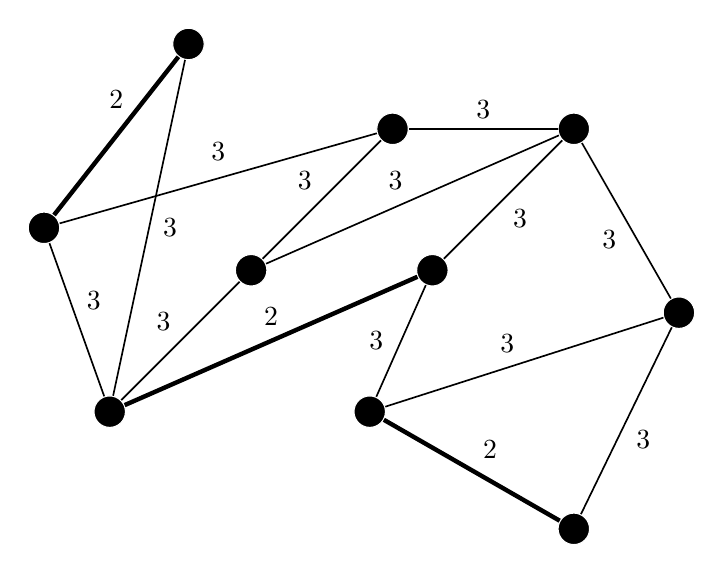
\begin{tikzpicture}[auto, node distance = 1.3in, on grid, state/.style = {circle, top color = black, bottom color = black, draw, white, text = black, minimum width = 4mm}]
	\node[state] (A) {};
	\node[state] (B) [below left = of A, xshift = 0.5cm] {};
	\node[state] (C) [below right = of B, xshift = -1.5cm] {};
	\node[state] (D) [node distance = 1in, above right = of C] {};
	\node[state] (E) [node distance = 1in, above right = of D] {};
	\node[state] (F) [right = of E, xshift = -1cm] {};
	\node[state] (G) [node distance = 1in, below left = of F] {};
	\node[state] (H) [node distance = 1in, below left = of G, xshift = 1cm] {};
	\node[state] (I) [below right = of F, xshift = -1cm] {};
	\node[state] (J) [node distance = 2in, below = of F] {};
	\draw[ultra thick] (A) -- node[above = 0.2cm]{2} (B);
	\draw[semithick] (B) -- node[auto]{3} (C);
	\draw[semithick] (A) -- node[right = 0.05cm]{3} (C);
	\draw[semithick] (B) -- node[above = 0.1cm]{3} (E);
	\draw[semithick] (C) -- node[auto]{3} (D);
	\draw[semithick] (D) -- node[auto]{3} (E);
	\draw[semithick] (D) -- node[auto]{3} (F);
	\draw[semithick] (E) -- node[auto]{3} (F);
	\draw[ultra thick] (C) -- node[above = 0.05cm]{2} (G);
	\draw[semithick] (F) -- node[auto]{3} (G);
	\draw[semithick] (G) -- node[left = 0.1cm]{3} (H);
	\draw[semithick] (H) -- node[auto]{3} (I);
	\draw[ultra thick] (H) -- node[auto]{2} (J);
	\draw[semithick] (I) -- node[auto]{3} (J);
	\draw[semithick] (I) -- node[auto]{3} (F);
	\end{tikzpicture}
\end{center}

Avem că toate muchiile de cost minim $c=2$ vor fi incluse într-un arbore parțial de cost minim, dar cum restul muchiilor sunt de cost $c=3 \Rightarrow$ există mai mulți $T \in \text{{\calligra T}}_G$ de cost minim care au $M \subset E(T) \Rightarrow$ afirmația \textbf{a)} este falsă.

\textbf{III}: Dacă interpretăm afirmația \textbf{a)} ca "Oricare $m \in M$ este conținut într-un arbore parțial de cost minim.", atunci, din maniera de alegere a algoritmului lui Kruskal (după sortarea tuturor muchiilor, oricare dintre cele cu cost minim poate fi luată și adăugată în APM, întrucât sigur nu se va crea un ciclu, fiindcă ar fi prima muchie) $\Rightarrow \forall m \in M$ va apărea într-un $T \in \text{{\calligra T}}_G$ de cost minim $\Rightarrow$ afirmația \textbf{a)} este adevărată.

\subsection{b)}

Fie $C$ un circuit în $G$ și $m \in E(C)$ o muchie de cost minim unică pe $C$.

Conform afirmației de la \textbf{b)}, ar trebui ca din ipoteză să rezulte că $m \in T^*, \forall T^* \in \text{{\calligra T}}_G$ de cost minim. Totuși, în exemplul de mai jos:

\begin{center}
	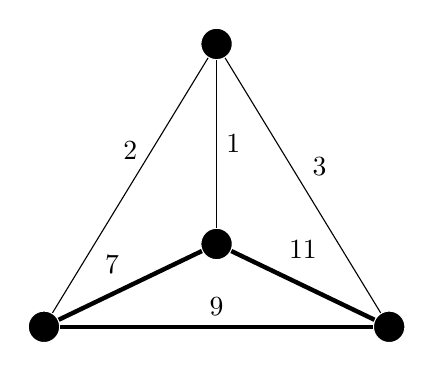
\begin{tikzpicture}[auto, node distance = 2in, on grid, state/.style = {circle, top color = black, bottom color = black, draw, white, text = black, minimum width = 4mm}]
	\node[state] (A) {};
	\node[state] (B) [below left = of A,xshift=1.4cm] {};
	\node[state] (D) [below right = of A,xshift=-1.4cm] {};
	\node[state] (C)[node distance = 1in,below = of A] {} ;
	\draw (A) -- node[above = 0.2cm]{2} (B);
	\draw (A) -- node[auto]{3} (D);
	\draw (A) -- node[auto]{1} (C);
	\draw[ultra thick] (B) -- node[auto]{7} (C);
	\draw[ultra thick] (B) -- node[auto]{9} (D);
	\draw[ultra thick] (C) -- node[above = 0.2cm] {11} (D);
	\end{tikzpicture}
\end{center}

Dacă luăm $C$ ca fiind circuitul îngroșat, atunci muchia sa $m$ de cost minim $c(m) = 7$ nu aparține $T^*, \forall T^* \in \text{{\calligra T}}_G$ de cost minim. Astfel, avem că afirmația \textbf{b)} este falsă.
\subsection{c)}

Fie $m \in E(G)$ o muchie care $\in E(T^*), T^* \in \text{{\calligra T}}_G$ de cost $c$ minim. $T^* - m$ conține subarborii $T', T''$. Considerăm $A = \left \{ uv \in E(G) | u \in V(T'), V \in V(T'')\right \}$ o tăietură a.î. $m \in A$.

Presupunem prin reducere la absurd că $\exists m' \in A$ a.î. $c(m') < c(m) \Rightarrow T^*-m+m'$ are costul mai mic decât $T^* \Rightarrow T^* \in \text{{\calligra T}}_G$ nu este de cost $c$ minim (contradicție) $\Rightarrow$ presupunerea făcută este falsă $\Rightarrow m$ este de cost minim în $A$. 

Conform celor de mai sus $\Rightarrow$ afirmația \textbf{c)} este adevărată.

\section{Problema 2}

\subsection{a)}

Presupunem că $H$ este $c$-extensibil, $H$ subgraf conex al lui $G$, $G$ conex. Atunci avem $T^*_H = \left(V(H), E(H) \cap E(T^*)\right) \in \text{{\calligra T}}_H$, unde $T^* \in \text{{\calligra T}}_G$ este de cost $c$ minim. Din $T^*_H\in \text{{\calligra T}}_H$ și $E(T^*_H)=E(H)\cap E(T^*) \Rightarrow T^*_H$ este format din $|V(H)|-1$ muchii ale lui $T^*$.

Presupunem prin reducere la absurd că $\exists T'_H \in \text{{\calligra T}}_H$ de cost minim $c' < c(T^*_H)$. Dar $E(T^*_H) \subseteq E(T^*) \Rightarrow \exists T' \in \text{{\calligra T}}_G, T'_H \subseteq T'$ a.î.  $c(T') < c(T^*) \Rightarrow T^*$ nu este arbore parțial de cost minim (contradicție) $\Rightarrow$ presupunerea făcută este falsă $\Rightarrow T^*_H \in \text{{\calligra T}}_H$ este de cost $c$ minim.

\subsection{b)}

Asamblarea unui arbore parțial de cost minim al lui $H$ cu un arbore parțial de cost minim al lui $G_{H}$ ar presupune găsirea a două mulțimi de muchii $S_1 \subseteq E(H)$  și $S_2 \subseteq E(G_{H})$, astfel încât reunuinea lor să formeze un arbore parțial de cost minim al lui $G$: să fie un graf conex cu n-1 muchii (unde $n=|V|$), fără cicluri, iar suma costurilor de pe muchii este minimă.

Fie $T^{*}$ un arbore parțial de cost minim oarecare din graful $G=(V,E)$. Din $a)$ $\Rightarrow T_{H}^{*}$ e un arbore parțial de cost minim al lui $H$, dar muchiile lui $T_{H}^{*}$ au fost luate ca fiind intersecția muchiilor subgrafului conex $H$ cu muchiile unui arbore parțial de cost minim $T^{*}$ din $G$, deci $E(T_{H}^{*}) \subseteq E(T^{*})$, deci putem lua $S_1 = E(T_{H}^{*})$.

Prin contractarea muchiilor subgrafului conex $H$ al lui $G$ într-un singur nod, să-l notăm cu $u$ vom obține un multigraf în care toate muchiile care intrau în subgraful $H$ vor intra acum în nodul $u$ (muchiile își păstrează costul). Fie $T'^{*}$ un arbore parțial de cost minim din $G_{H}$. Știm că $u \in V(T'^{*})$, deci $d_{T'^{*}}(u) \in \{1,2\}$ (poate fi frunză sau poate fi nod interior, însă în ambele cazuri există un drum de lungime minimă de la $u$ la $v, \forall v \in V(T'^{*})$, deci putem lua $S_2 = E(T'^{*})$.

\textbf{Afirmație:} Reuniunea mulțimilor $S_1$ și $S_2$, construite ca mai sus, formează un arbore parțial de cost minim al lui $G$.
 
\textbf{Demonstrație:} Muchiile din $S_1$ au fost luate ca fiind intersecția subgrafului $H$ cu muchiile unui arbore parțial de cost minim oarecare al lui $G$, iar muchiile din $S_2$ aparțin unui arbore parțial de cost minim din $G_{H}$, deci prin decontractarea muchiilor din $H$ vom avea că există 1 sau 2 noduri (în functie de $d_{T'^{*}}(u)$, unde $u$ este nodul obținut prin contractarea lui $H$) din $V(H)$ adiacente cu muchii din $S_2$, ceea ce ar face ca reuniunea muchiilor $S_1$ și $S_2$ să fie un graf conex, cu $|S_1| + |S_2| = |V|-1$, deci și aciclic, iar prin construcție costul muchiilor din cele 2 mulțimi au suma minimă posibilă, deci asamblarea lor ar forma un arbore parțial de cost minim al lui $G$.

\section{Problema 3}

\textbf{I.(i) $\Rightarrow$ (ii)}: Pesupunem prin reducere la absurd că $G$ este neconex. Din faptul că $G$ nu este nul (\textbf{(i)}) $\Rightarrow |E(G)| \neq 0\ (|E(G)| > 0)$, adică avem cel puțin 2 componente conexe. Dacă luăm $x,y$ două noduri, $x \in S, y \in T$ din componente conexe diferite, pe care le eliminăm apoi din $G$, vom obține un cuplaj $M'$ de cardinal maxim $< |G-\{x,y\}|/2$. Dar $G-\{x,y\}$ are cuplaj perfect,$\forall x \in S, \forall y \in T$ (\textbf{(i)}) $\Rightarrow |M'| = |G-\{x,y\}|/2$ (contradicție) $\Rightarrow$ presupunerea făcută este falsă $\Rightarrow G$ este conex. 

Din faptul că G este conex, iar $G-\{x,y\}$ are cuplaj perfect,$\forall x \in S, \forall y \in T \Rightarrow \forall m \in E(G)$ aparține unui cuplaj perfect.

\textbf{II.(ii) $\Rightarrow$ (iii)}: Din $G$ conex (\textbf{(ii)}) $\Rightarrow G$ nu este nul.

Presupunem prin reducere la absurd că $|S| \neq |T|$. Vom avea că $\forall e \in E(G)$ aparține unui cuplaj $M \in \text{{\calligra M}}_G$ de cardinal $ < |G|/2$. Dar $\forall e \in E(G)$ aparține unui cuplaj perfect (\textbf{(ii)}), adică $|M| = |G|/2$ (contradicție) $\Rightarrow$ presupunerea făcută este falsă $\Rightarrow |S| = |T|$. 

Din $\forall e \in E(G)$ aparține unui cuplaj perfect $\Rightarrow \exists M \in \text{{\calligra M}}_G$ de cardinal $|G|/2$ care să satureze $S \xRightarrow{Hall} |N_G(A)| \geq |A|, \forall A \subseteq S$. Dacă luăm $A \subsetneq S, A \neq \varnothing$, din faptul că $G$ este conex și $\forall e \in E(G)$ aparține unui cuplaj perfect $\Rightarrow |N_G(A)| > |A|$.

\textbf{III.(iii) $\Rightarrow$ (i)}: Din $G$ nenul, $|S| = |T|$ și $|N_G(A)| > |A|, \varnothing \neq A \subsetneq S \Rightarrow$ dacă eliminăm $\forall x \in S, \forall y \in T$, vom obține graful bipartit $G-\{x,y\}$ cu $|S\setminus \{x\}| = |T\setminus \{y\}|$ și $|N_{G-\{x,y\}}(A)| \geq |A|, \forall A \subseteq \left(S\setminus \{x\} \right) \xRightarrow{Hall} \exists$ un cuplaj $M$ în $G-\{x,y\}$ care să satureze $S\setminus \{x\}$. Dar  cum $|S\setminus \{x\}| = |T\setminus \{y\}|, \forall x \in S, \forall y \in T \Rightarrow$  cuplajul $M \in \text{{\calligra M}}_{G-\{x,y\}}$ este de cardinal $|G-\{x,y\}|/2 \Rightarrow G-\{x,y\}$ are un cuplaj perfect, $\forall x \in S, \forall y \in T$.

Din (\textbf{I}), (\textbf{II}) și (\textbf{III}) $\Rightarrow$ afirmațiile \textbf{(i)}, \textbf{(ii)} și \textbf{(iii)} sunt echivalente.

\section {Problema 4}

Următoarele observații vor fi folosite în mai multe subpuncte ce urmează a fi rezolvate:

Fie $G = (V,E)$ un graf $p$-regulat bipartit. Pentru $G$, vom nota cele 2 mulțimi stabile cu $S$ și $T$.

\begin{enumerate}[I.]
	\item Un graf este p-regulat dacă toate nodurile sale au gradul p.
	\item Un graf este bipartit dacă nu conține circuite de lungime impară. Din această observație $\Rightarrow$ că toate circuitele găsite de algoritm în timpul iterațiilor while vor avea număr par de muchii, iar cele 2 cuplaje $M_1$ și $M_2$ vor avea mereu aceeași structură (pe baza unui circuit): fie $C$ un circuit de lungime $k$ a cărui muchii sunt, în ordine: $e_1$, $e_2$, ... $e_k$; $M_1$ va conține muchiile $e_1$, $e_3$, ... $e_{k-1}$ iar $M_2$ va conține muchiile $e_2$, $e_4$, ... $e_k$, orice altă distribuire a acestora făcând ca $M_1$ și $M_2$ să încalce proprietățile cuplajului.
	
	\begin{figure}[h!]
	\centering
	\subfloat[]{
		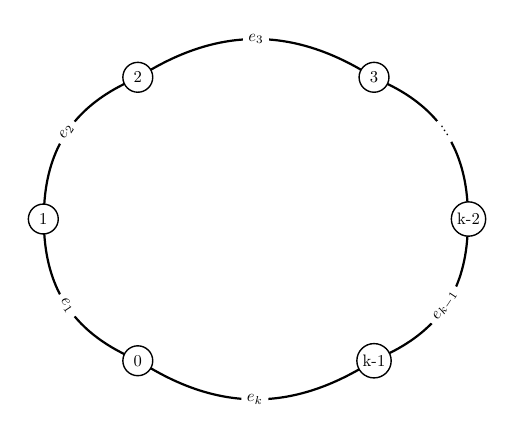
\begin{tikzpicture}[scale=0.6,transform shape]
		\Vertex[x=1,y=0]{0}
		\Vertex[x=-1,y=3]{1}
		\Vertex[x=1,y=6]{2}
		\Vertex[x=6,y=6]{3}
		\Vertex[x=8,y=3]{k-2}
		\Vertex[x=6,y=0]{k-1}
		\tikzstyle{LabelStyle}=[fill=white,sloped]
		\tikzstyle{EdgeStyle}=[bend left]
		\Edge[label=$e_1$](0)(1)
		\Edge[label=$e_2$](1)(2)
		\Edge[label=$e_3$](2)(3)
		\Edge[label=$...$](3)({k-2})
		\Edge[label=$e_k$]({k-1})(0)
		\tikzstyle{EdgeStyle}=[bend right]
		\Edge[label=$e_{k-1}$]({k-1})({k-2})
		\end{tikzpicture}
	}
  	\caption{Observația II, Etichetarea muchiilor unui circuit.}
	\end{figure}

	
	\item Orice graf $p$-regulat bipartit admite cuplaj perfect. (adică pentru orice graf $G$ care respectă specificațiile va exista o submulțime $M \subseteq E$ care reprezinte un cuplaj perfect).
	
	\textbf{Demonstrație} Conform Teoremei lui Hall, pentru un graf bipartit $G=(S,T,E)$, există un cuplaj în care G saturează toate nodurile din $S$ dacă și numai dacă
	$$ |N_G(A)| \geq |A|, \forall A \subseteq S $$
	Fiindcă G e $p$-regulat, numărul de muchii dintre $A$ și $N_G(A)$ este $k \cdot |A|$, numărul de muchii incidente cu nodurile din $N_G(A)$ este $k \cdot |N_G(A)|$, și are loc inegalitatea $ k \cdot |N_G(A)| \geq k \cdot |A| $ (fiindcă toate nodurile din $N_G(A)$ conțin ca noduri adiacente nodurile din $A$, și posibil altele în plus). Așadar $|N_G(A)| \geq |A|$, deci $G$ saturează toate nodurile din $S$. Dar $|S|$ = $|T|$, deci $G$ saturează și toate nodurile din $T$, deci $G$ admite cuplaj maxim.
	
\end{enumerate}

\subsection{a)}

Fie $n$ lungimea circuitului $C$ (numărul de muchii de pe circuit). Fiecare dintre cuplajele $M_{1}$ și $M_{2}$ va avea câte $n = k/2$ muchii. Vom nota cu $n_i$ $a(e), \forall e \in M_{1}$ și cu $m_i$ $a(e), \forall e \in M_{2}$. Înainte de iterația while $f(E^{+}) = X = n_1^2 + n_2^2 + ... + n_k^2 + m_1^2 + m_2^2 + ... + m_k^2$. După această iterație $n_i$ va crește cu 1 $\forall 1 \leq i \leq k$, și $m_i$ va scădea cu 1 $\forall 1 \leq i \leq k$, deci $ f(E^{+}) = Y = (n_1+1)^2 + (n_2+1)^2 + ... + (n_k+1)^2 + (m_1-1)^2 + (m_2-1)^2 + ... + (m_k-1)^2 $. Valoarea cu care se modifică $f(E^{+})$ după fiecare iterație este $MOD = Y - X = (n_1+1)^2 + (n_2+1)^2 + ... + (n_k+1)^2 + (m_1-1)^2 + (m_2-1)^2 + ... + (m_k-1)^2 - (n_1^2 + n_2^2 + ... + n_k^2 + m_1^2 + m_2^2 + ... + m_k^2) = (n_1^2 + 2 \cdot n_1 + 1) + (n_2^2 + 2 \cdot n_2 + 1) + ... + (n_k^2 + 2 \cdot n_k + 1) + (m_1^2 - 2 \cdot m_1 + 1) + (m_2^2 - 2 \cdot m_2 + 1) + ... + (m_k^2 - 2 \cdot m_k + 1) - (n_1^2 + n_2^2 + ... + n_k^2 + m_1^2 + m_2^2 + ... + m_k^2) = 2 \cdot (n_1 + n_2 + ... + n_k - m_1 - m_2 - ... - m_k) + (1 + 1 + ... + 1) = 2 \cdot (n_1 + n_2 + ... + n_k - m_1 - m_2 - ... - m_k) + k$. Din modul în care au fost alese cuplajele $M_1$ și $M_2$, rezultatul parantezei $(n_1 + n_2 + ... + n_k - m_1 - m_2 - ... - m_k)$ este pozitiv (fiindcă $a(M_2) \leq a(M_1)$), deci $MOD \geq k$, deci $MOD \geq |C|$, deci după fiecare iterație $while$, $f(E^{+})$ va crește cu cel puțin $|C|$ față de valoarea anterioară.

\subsection{b)}

Înainte de prima iterație $while$, $a(e)=1, \forall e \in E$, iar fiecare nod este incident cu exact $p$ muchii, deci egalitatea $ \sum_{uv \in E^{+}} a(uv) = p $ are loc pentru orice nod $u$.

Fie $t$ numărul iterației curente $while$. Putem împărți nodurile în două categorii: noduri ce se află pe circuitul $C$ selectat, și noduri care nu se află pe circuit.

Fie $u$, pe rând, fiecare nod din prima categorie. $u$ este incident cu exact 2 muchii $e_{1}$ și $e_{2}$ (fiindcă orice nod de pe un circuit are gradul 2), iar $e_{1}$ și $e_{2}$ se află în cuplaje diferite, deci putem presupune, fără a restrânge generalitatea, că $e_{1} \in M_{1}$ și $e_{2} \in M_{2}$. În urma execuției instrucțiunilor din iterația while, valoarea a($e_{1}$) a crescut cu 1, iar valoarea a($e_{2}$) a scăzut cu 1. Fie $x = \sum_{uv \in E^{+}} a(uv) = p$ pentru iterația $t-1$ și $y = \sum_{uv \in E^{+}} a(uv) $ pentru iterația $t$. Fiindcă singurele muchii care au afectat valoarea lui $x$ sunt $e_{1}$ și $e_{2}$, înseamnă că $y = x + 1 - 1 = p$, deci și după iterația $t$ $ \sum_{uv \in E^{+}} a(uv) = p $ pentru nodul curent $u$ $(1)$.

Fie $v$, pe rând, fiecare nod din a doua categorie (care nu se află pe circuitul $C$). Știm că pentru iterația $t-1$ egalitatea $ \sum_{vw \in E^{+}} a(vw) = p $ are loc, iar în timpul iterației $t$ nici unei muchii incidente cu $v$ nu i se va schimba valoarea (pentru că altfel $v$ s-ar fi aflat pe circuit), deci egalitatea are în continuare loc $(2)$.

$(1) + (2) \Rightarrow$ pentru orice nod $u \in V$, dupa fiecare iterație $while$, $ \sum_{uv \in E^{+}} a(uv) = p $.

\subsection{c)}

Dacă în timpul algoritmului, la o iterație $t$, în graful $G^{+}$, un nod $u$ din graf e adiacent cu o muchie $e = uv$ ce are $a(e) = p$, înseamnă că gradul acelui nod este 1 (adică muchia $e$ este singura muchie cu care $u$ este incident), deci acest nod nu se va putea afla pe un circuit $\Rightarrow$ $u$ va fi ignorat, deci muchiile cu $a(e) = p$ nu vor mai fi luate în considerare. De asemenea, $ \nexists e \in E^{+}$ în $G^{+} = (V,E^{+})$ cu proprietatea că $a(e) = 0$ (din modul în care e construit $E^{+}$). Am văzut conform observației III că graful $G$ admite un cuplaj perfect (fiindcă este $p$-regulat bipartit), iar din structura lui, acesta va conține cicluri până când nu au fost saturate toate nodurile. Fiecare muchie $e$ care ajunge să aibă $a(e) = p$ va satura 2 noduri din $G$, iar algoritmul va continua cât timp există muchii cu $a(e) \neq p$ ( cât timp există cicluri), deci la final $E^{+}$ va conține muchii care saturează câte 2 noduri, deci muchiile unui cuplaj perfect al lui $G$.

\subsection{d)}

Din $(c) \Rightarrow $ algoritmul se va opri când va găsi o submulțime de muchii din $E$ care să formeze un cuplaj perfect al lui $G$, deci numărul de iterații while este finit. 

De asemenea din $(c)$ știm că $ a(e) = p, \forall e \in E^{+} $ $(1)$. Numărul de muchii din cuplajul perfect al lui $G$ este $x = |V|/2$, deci la finalul algoritmului $|E^{+}| = |V|/2$ $(2)$. $(1) + (2) \Rightarrow$ $E^{+}$ conține $|V|/2$ muchii, fiecare având $a(e) = p$. Deci dacă $n=|V|$ avem că $f(E^{+})= p^2 + p^2 + ... + p^2 = (|V|/2) \cdot p^2 = (n \cdot p^2)/2$. În plus, cum fiecare nod din graf este incident cu $p$ muchii, înseamnă că numărul de muchii $m$ e egal cu $(n \cdot p)/2$ (fiindcă o muchie e adiacentă cu 2 noduri), deci $f(E^{+})= (n \cdot p^2)/2 = p \cdot m$. Am demonstrat la $a)$ că la fiecare iterație $while$ valoarea $f(E^{+})$ va crește cu cel puțin $|C|$ (lungimea circuitului găsit), iar tocmai am demonstrat că în final $f(E^{+})=pm$. Deci dacă la fiecare iterație valoarea lui $f(E^{+})$ crește cu exact $|C|$, atunci în final suma lungimilor tuturor circuitelor va fi $p \cdot m$ (mai mult de atât nu poate fi), iar în cazul în care $f(E^{+})$ crește cu mai mult de $|C|$, atunci suma lungimilor tuturor circuitelor se va micșora. 

\subsection{e)}

După cum am vazut și la $c)$, numai acele muchii $e$ cu $a(e) \neq p$ pot fi luate în considerare atunci când se caută un circuit $C$ (cele care au ajuns să aibă $a(e) = p$ sau $a(e) = 0$ sunt complet ignorate). În plus, tot din $c)$ am văzut că dacă un nod $u$ este adiacent cu cel puțin 2 muchii, atunci el sigur se află pe un circuit și deci făcând o parcurgere dfs din acel nod și mergând doar pe muchii $e$ care au $a(e) \neq p$ vom găsi o muchie de întoarcere (deci vom găsi un circuit). Aceste observații ne dau și algoritmul care găsește un circuit în complexitate $O(|C|)$: fie $s$ un nod care e adiacent cu o muchie $e$ ce are $a(e) \neq p$, se face un dfs și se parcurg numai muchii ce au $a(muchie) \neq p$ până la găsirea unei muchii de întoarcere $uv$. După găsirea muchiei de întoarcere, trebuie eliminate muchiile incidente cu nodurile de pe lanțul de la $s$ până la părintele nodului $v$ (cel către care a fost găsită muchia de întoarcere). 

\begin{algorithm}
	\begin{algorithmic}[1]
		\State $C \gets \varnothing$;
		\For {$(v \in V)$}
				\State $visited[v] \gets false$;
				\State $before[v] \gets NULL$;
		\EndFor
		\State $S \gets stivaVida()$;
		\State $push(S,s)$; // s e un nod care e incident cu o muchie ce are $a(e) \neq p$
		\While {$ (true) $}
			\State $ u \gets top(S)$;
			\State $ visited[u] \gets true$;
			\If {$((v \gets next[A[u]]) \neq NULL)$}
				\If {$(visited[v] = false)$}
					\State $push(S,v)$;
					\State $A'[v] \gets A'[v] \backslash \{u\}$;
					\State $E' \gets E' \cup \{uv\}$;
				\Else
					\State $E' \gets E' \cup \{uv\}$;
					\State $child \gets v$;
					\State $father \gets before[v]$;
					\State break;
				\EndIf
			\EndIf
		\EndWhile
		\While {$(father \neq NULL)$}
			\State $C \gets C$  $\backslash \{father-child\}$; // sterg muchiile care nu sunt pe circuit
			\State $ child \gets father$; $father \gets before[father]$;
		\EndWhile
		\State $return$ $C$;
	\end{algorithmic}
\end{algorithm}	

\subsection{f)}

Știm conform subpunctului $d)$ că suma lungimilor tuturor circuitelor procesate este cel mult $pm$, iar din $e)$ $\Rightarrow$ la fiecare iterație găsirea unui circuit $C$ are complexitate liniară în raport cu dimensiunea circuitului. Existența instrucțiunii $for$ din cadrul buclei $while$ nu va înrăutăți asimptotic complexitatea algoritmului, întrucât în cadrul acelui $for$ sunt parcurse muchiile de pe circuit, despre care știm că vor fi maxim $pm$ de-a lungul execuției programul $(1)$. În plus, instrucțiunile dinainte buclei $while$ au complexitatea $\mathcal{O}(m)$ (sunt parcurse muchiile de 2 ori), deci nu au impact asupra complexității $(2)$. $(1)$ $+$ $(2)$ $\Rightarrow$ operațiile dominante din algoritm sunt procesarea muchiilor de pe circuite, numărul lor fiind maxim $p \cdot m$, deci complexitatea algoritmului este $\mathcal{O}(pm)$.

\end{document}